%\documentclass{article}
\documentclass[acmlarge,nonacm,natbib=false]{acmart}
\usepackage{graphicx} % Required for inserting images
%\usepackage{biblatex} %Imports biblatex package
\RequirePackage[
datamodel=acmdatamodel,
style=acmnumeric, % use style=acmauthoryear for publications that require it
]{biblatex}
\addbibresource{biblio.bib}
\usepackage{url}
\usepackage{hyperref}
%\usepackage[spanish]{babel}
\usepackage[utf8x]{inputenc}
\usepackage{tikz}
\usepackage{amsmath}
\usepackage{float}
\tikzstyle{vertexb}=[auto=left,circle,fill=blue!25,minimum size=15pt,inner sep=0pt]
\tikzstyle{vertexr}=[auto=left,circle,fill=red!25,minimum size=15pt,inner sep=0pt]
\tikzstyle{vertexg}=[auto=left,circle,fill=green!25,minimum size=15pt,inner sep=0pt]
\tikzstyle{vertexy}=[auto=left,circle,fill=yellow!25,minimum size=15pt,inner sep=0pt]

\date{April 2024}
\raggedbottom
\begin{document}
\title{Estudi de la influència de les condicions inicials en la propagació de una pandemia}
\author{Guillem Béjar Riera}
\author{Miquel Calvo Simó}
\author{Jan Marc Extremera Garcia}
\author{Marc Vilà Tintiñà}
\begin{abstract}
En aquest treball es pretén explicar el funcionament d'un dels models diferencials més bàsics i fonamentals per a la modelació del creixement d'una malaltia infecciosa. Es comença detallant alguns conceptes teòrics on es mostra l'estructura i característiques del model i posteriorment s'inclou un estudi per a determinar l'impacte de la vacunació en l'evolució d'aquesta.

\midbreak

\noindent En més detall, s'introdueix la base, definició i paràmetres del model. S'esmenten les aplicacions més rellevants d'aquest i els beneficis que se'n poden extreure. Se'n fa una anàlisi per a veure com afecten les mesures preventives posant d'exemple l'impacte del confinament en l'evolució d'una pandèmia amb uns certs paràmetres inicials. I finalment, s'analitza els efectes de la vacunació i el benefici que presenta.

\end{abstract}

\maketitle

\pagebreak

\tableofcontents
\listoffigures

\pagebreak


\section{Model SIR}
El model SIR és dels models matemàtics més senzills que poden descriure i modelitzar una pandèmia d'una malaltia infecciosa amb bastant rigorositat. El model es va anar desenvolupant al llarg del segle XX, però les aportacions més importants les van realitzar Ross~\cite{ross}, Kermark, McKendrik~\cite{kmk} i Kendall~\cite{kendall}. El model es caracteritza per els 3 estats possibles en que pot estar un individu:
\begin{itemize}
    \item Persones susceptibles (S): Persones que encara no s’han infectat de la malaltia i no tenen cap mena d’immunitat.
    \item Persones infectades (I): Persones que han passat de l’etapa d’infecció i incubació i ja estan experimentant els efectes de la malaltia. Aquests individus tenen capacitat d’infectar persones susceptibles.
    \item Persones recuperades (R): Persones que han superat la malaltia i ja no posseeixen capacitat infecciosa. A més ja no es poden tornar a infectar, ja que han adquirit immunitat a l'agent causant de la malaltia.
\end{itemize}

\bigbreak

\noindent En aquest model es fan moltes aproximacions i s'obvien molts detalls, ja que sinó seria molt més complex. Per exemple, el grup R, inclou les persones que han mort per culpa de la malaltia. També es considera que la població és constant, és a dir, el nombre de naixements és igual al de les morts per culpa de la malaltia que es modela i les morts causades per altres factors. A més se suposa que la immunitat és 100\% efectiva i no perd eficàcia durant el temps. En alguns patògens es pot estar en l'estat de portador, on la persona no està infectada però encara té capacitat infecciosa~\cite{wikicme}

\medbreak

El model més bàsic és composa d’aquestes 3 EDOs:

\smallbreak

\begin{math}\frac{dS}{dt}=-\beta SI\end{math}

\begin{math}\frac{dI}{dt}=\beta SI - \gamma I\end{math}

\begin{math}\frac{dR}{dt}=\gamma I\end{math}

\medbreak

\noindent On S representa el nombre de persones susceptibles, I el nombre d'infectades i R el de recuperades. Tots aquests valors s'han normalitzat amb el valor de població. \begin{math}\beta\end{math} representa la quantitat de persones amb qui un infectat interactua multiplicat per la probabilitat de transmissió de la malaltia. \begin{math}\gamma\end{math} és la inversa del temps mitja que tarda un infectat en recuperar-se. El model és determinista, és a dir, les mateixes condicions inicials portaran al mateix resultat, ja que no té cap element que indueix caos matemàtic. 
\medbreak
\noindent Un cop tenim definits \begin{math}\beta\end{math} i \begin{math}\gamma\end{math}, podem calcular \begin{math}R_0\end{math} o Nombre reproductiu bàsic, amb l’expressió \begin{math}\frac{\beta}{\gamma}\end{math}. Aquest valor determina a quants individus sans pot infectar un infectat. A més, un cop tenim definit \begin{math}R_0\end{math}, podem definir \begin{math}R_e\end{math} o nombre reproductiu efectiu~\cite{siruab}. Aquest nombre es molt semblant a \begin{math}R_0\end{math} però es lleugerament més exacte, ja que només te en compte la part de la població que es pot infectar, els susceptibles. \begin{math}R_e\end{math} es calcularia de la següent forma: \begin{math}R_e=\frac{S(0)}{N}R_0\end{math}. On S(0) es la població inicial de susceptibles i N la població inicial. Amb aquest valor podem determinar com evolucionarà un brot.

Propietats de \begin{math}R_e\end{math}:
\begin{itemize}
    \item Si \begin{math}R_e\end{math}<1 , l’infecció serà molt lenta i molt dificilment es convertirà en pandèmia. (Veure Fig2)
    
    \item Si \begin{math}R_e\end{math}=1, els infectats augmentaran de forma exponencial seguint la funció \begin{math}2^t\end{math} on \begin{math}t\in \mathbb{N}^+\end{math} representa el temps, mesurat en dies. 
     (Veure Fig3)
    
    \item En cas que sigui major que 1, hi haurà una epidèmia “descontrolada” ja que els casos creixeran de forma exponencial, encara més rapid que l’exponencial a \begin{math}R_e\end{math}=1~\cite{siruab}. (Veure Fig4)

\end{itemize}

\begin{math}R_0=\frac{\beta}{\gamma}\end{math}

\begin{math}S=\frac{2\gamma}{\beta}\end{math}

\begin{math}S<\frac{2\gamma}{\beta}\end{math}

\begin{math}S>\frac{2\gamma}{\beta}\end{math}

\begin{math}S<R_0^{-1}\end{math}

\begin{math}S=R_0^{-1}\end{math}

\begin{math}S>R_0^{-1}\end{math}

\begin{figure}[h!]
\begin{center}
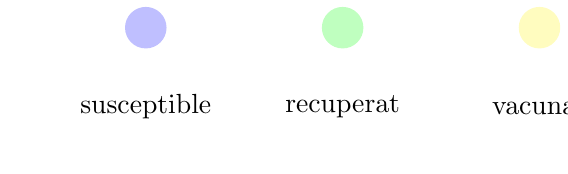
\begin{tikzpicture}[x=0.5cm,y=0.5cm]
    \useasboundingbox (2,0) rectangle (15,3);
    \node[vertexr] (n1) at (0,3)  {};
    \node[vertexb] (n2) at (5,3)  {};
    \node[vertexg] (n3) at (10,3) {};
    \node[vertexy] (n4) at (15,3) {};
    \node (en1) at (0,1)  {infectat};
    \node (en2) at (5,1)  {susceptible};
    \node (en3) at (10,1) {recuperat};
    \node (en4) at (15,1) {vacunat};
  
\end{tikzpicture} 

\end{center}

\caption{Tipus de nodes}
\end{figure}

\begin{figure}[h!]
\begin{center}
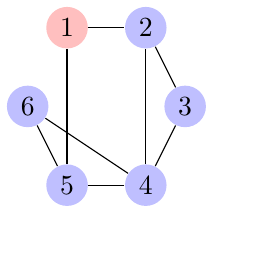
\begin{tikzpicture}[x=0.5cm,y=0.5cm]
    \useasboundingbox (2,-2) rectangle (7.5,3);
    \node[vertexr] (n1) at (3,3)  {1};
    \node[vertexb] (n2) at (5,3)  {2};
    \node[vertexb] (n3) at (6, 1) {3};
    \node[vertexb] (n4) at (5, -1) {4};
    \node[vertexb] (n5) at (3, -1) {5};
    \node[vertexb] (n6) at (2, 1) {6};
    
  
    \foreach \from/\to in {n1/n2,n1/n5,n2/n3,n2/n4,n3/n4,n4/n5,n4/n6,n5/n6}
    \draw (\from) -- (\to);
\end{tikzpicture}
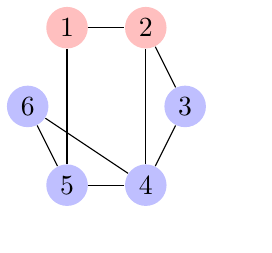
\begin{tikzpicture}[x=0.5cm,y=0.5cm]
    \useasboundingbox (2,-2) rectangle (7.5,3);
    \node[vertexr] (n1) at (3,3)  {1};
    \node[vertexr] (n2) at (5,3)  {2};
    \node[vertexb] (n3) at (6, 1) {3};
    \node[vertexb] (n4) at (5, -1) {4};
    \node[vertexb] (n5) at (3, -1) {5};
    \node[vertexb] (n6) at (2, 1) {6};
    
    \foreach \from/\to in {n1/n2,n1/n5,n2/n3,n2/n4,n3/n4,n4/n5,n4/n6,n5/n6}
    \draw (\from) -- (\to);
\end{tikzpicture} 
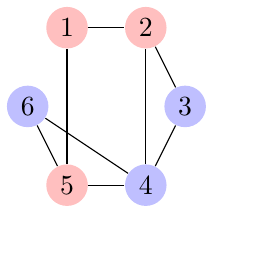
\begin{tikzpicture}[x=0.5cm,y=0.5cm]
    \useasboundingbox (2,-2) rectangle (7.5,3);
    \node[vertexr] (n1) at (3,3)  {1};
    \node[vertexr] (n2) at (5,3)  {2};
    \node[vertexb] (n3) at (6, 1) {3};
    \node[vertexb] (n4) at (5, -1) {4};
    \node[vertexr] (n5) at (3, -1) {5};
    \node[vertexb] (n6) at (2, 1) {6};
    
    \foreach \from/\to in {n1/n2,n1/n5,n2/n3,n2/n4,n3/n4,n4/n5,n4/n6,n5/n6}
    \draw (\from) -- (\to);
\end{tikzpicture}

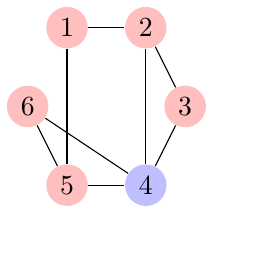
\begin{tikzpicture}[x=0.5cm,y=0.5cm]
    \useasboundingbox (2,-2) rectangle (7.5,3);
    \node[vertexr] (n1) at (3,3)  {1};
    \node[vertexr] (n2) at (5,3)  {2};
    \node[vertexr] (n3) at (6, 1) {3};
    \node[vertexb] (n4) at (5, -1) {4};
    \node[vertexr] (n5) at (3, -1) {5};
    \node[vertexr] (n6) at (2, 1) {6};
    
    \foreach \from/\to in {n1/n2,n1/n5,n2/n3,n2/n4,n3/n4,n4/n5,n4/n6,n5/n6}
    \draw (\from) -- (\to);
\end{tikzpicture} 
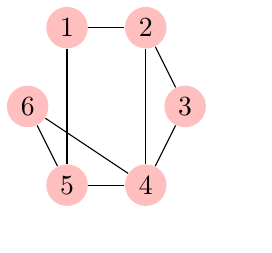
\begin{tikzpicture}[x=0.5cm,y=0.5cm]
    \useasboundingbox (2,-2) rectangle (7.5,3);
    \node[vertexr] (n1) at (3,3)  {1};
    \node[vertexr] (n2) at (5,3)  {2};
    \node[vertexr] (n3) at (6, 1) {3};
    \node[vertexr] (n4) at (5, -1) {4};
    \node[vertexr] (n5) at (3, -1) {5};
    \node[vertexr] (n6) at (2, 1) {6};
    
    \foreach \from/\to in {n1/n2,n1/n5,n2/n3,n2/n4,n3/n4,n4/n5,n4/n6,n5/n6}
    \draw (\from) -- (\to);
\end{tikzpicture} 

\end{center}

\caption{Seqüència d'infeccions amb \begin{math}R_e\end{math}<1 (Esquerra a dreta, dalt a baix) }\label{fig2}
\end{figure}

\begin{figure}[h!]
\begin{center}
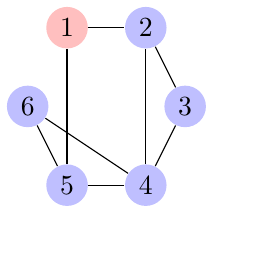
\begin{tikzpicture}[x=0.5cm,y=0.5cm]
    \useasboundingbox (2,-2) rectangle (7.5,3);
    \node[vertexr] (n1) at (3,3)  {1};
    \node[vertexb] (n2) at (5,3)  {2};
    \node[vertexb] (n3) at (6, 1) {3};
    \node[vertexb] (n4) at (5, -1) {4};
    \node[vertexb] (n5) at (3, -1) {5};
    \node[vertexb] (n6) at (2, 1) {6};
    
  
    \foreach \from/\to in {n1/n2,n1/n5,n2/n3,n2/n4,n3/n4,n4/n5,n4/n6,n5/n6}
    \draw (\from) -- (\to);
\end{tikzpicture}
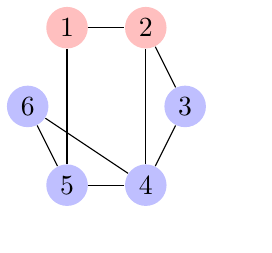
\begin{tikzpicture}[x=0.5cm,y=0.5cm]
    \useasboundingbox (2,-2) rectangle (7.5,3);
    \node[vertexr] (n1) at (3,3)  {1};
    \node[vertexr] (n2) at (5,3)  {2};
    \node[vertexb] (n3) at (6, 1) {3};
    \node[vertexb] (n4) at (5, -1) {4};
    \node[vertexb] (n5) at (3, -1) {5};
    \node[vertexb] (n6) at (2, 1) {6};
    
    \foreach \from/\to in {n1/n2,n1/n5,n2/n3,n2/n4,n3/n4,n4/n5,n4/n6,n5/n6}
    \draw (\from) -- (\to);
\end{tikzpicture} 
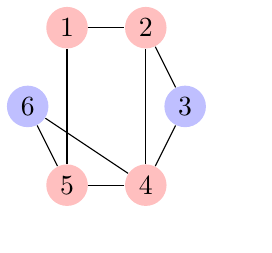
\begin{tikzpicture}[x=0.5cm,y=0.5cm]
    \useasboundingbox (2,-2) rectangle (7.5,3);
    \node[vertexr] (n1) at (3,3)  {1};
    \node[vertexr] (n2) at (5,3)  {2};
    \node[vertexb] (n3) at (6, 1) {3};
    \node[vertexr] (n4) at (5, -1) {4};
    \node[vertexr] (n5) at (3, -1) {5};
    \node[vertexb] (n6) at (2, 1) {6};
    
    \foreach \from/\to in {n1/n2,n1/n5,n2/n3,n2/n4,n3/n4,n4/n5,n4/n6,n5/n6}
    \draw (\from) -- (\to);
\end{tikzpicture}
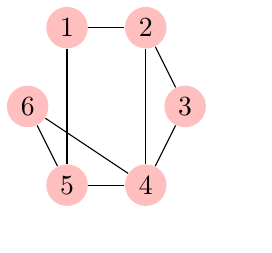
\begin{tikzpicture}[x=0.5cm,y=0.5cm]
    \useasboundingbox (2,-2) rectangle (7.5,3);
    \node[vertexr] (n1) at (3,3)  {1};
    \node[vertexr] (n2) at (5,3)  {2};
    \node[vertexr] (n3) at (6, 1) {3};
    \node[vertexr] (n4) at (5, -1) {4};
    \node[vertexr] (n5) at (3, -1) {5};
    \node[vertexr] (n6) at (2, 1) {6};
    
    \foreach \from/\to in {n1/n2,n1/n5,n2/n3,n2/n4,n3/n4,n4/n5,n4/n6,n5/n6}
    \draw (\from) -- (\to);
\end{tikzpicture} 

\end{center}

\caption{Seqüència d'infeccions amb \begin{math}R_e\end{math}=1 (Esquerra a dreta)}\label{fig3}
\end{figure}

\pagebreak

\begin{figure}[h!]
\begin{center}
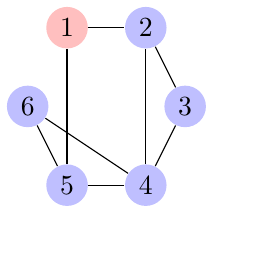
\begin{tikzpicture}[x=0.5cm,y=0.5cm]
    \useasboundingbox (2,-2) rectangle (7.5,3);
    \node[vertexr] (n1) at (3,3)  {1};
    \node[vertexb] (n2) at (5,3)  {2};
    \node[vertexb] (n3) at (6, 1) {3};
    \node[vertexb] (n4) at (5, -1) {4};
    \node[vertexb] (n5) at (3, -1) {5};
    \node[vertexb] (n6) at (2, 1) {6};
    
  
    \foreach \from/\to in {n1/n2,n1/n5,n2/n3,n2/n4,n3/n4,n4/n5,n4/n6,n5/n6}
    \draw (\from) -- (\to);
\end{tikzpicture}
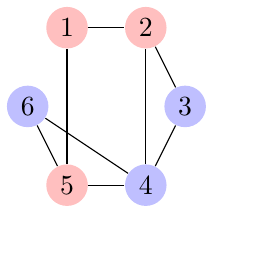
\begin{tikzpicture}[x=0.5cm,y=0.5cm]
    \useasboundingbox (2,-2) rectangle (7.5,3);
    \node[vertexr] (n1) at (3,3)  {1};
    \node[vertexr] (n2) at (5,3)  {2};
    \node[vertexb] (n3) at (6, 1) {3};
    \node[vertexb] (n4) at (5, -1) {4};
    \node[vertexr] (n5) at (3, -1) {5};
    \node[vertexb] (n6) at (2, 1) {6};
    
    \foreach \from/\to in {n1/n2,n1/n5,n2/n3,n2/n4,n3/n4,n4/n5,n4/n6,n5/n6}
    \draw (\from) -- (\to);
\end{tikzpicture}
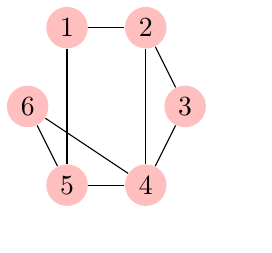
\begin{tikzpicture}[x=0.5cm,y=0.5cm]
    \useasboundingbox (2,-2) rectangle (7.5,3);
    \node[vertexr] (n1) at (3,3)  {1};
    \node[vertexr] (n2) at (5,3)  {2};
    \node[vertexr] (n3) at (6, 1) {3};
    \node[vertexr] (n4) at (5, -1) {4};
    \node[vertexr] (n5) at (3, -1) {5};
    \node[vertexr] (n6) at (2, 1) {6};
    
    \foreach \from/\to in {n1/n2,n1/n5,n2/n3,n2/n4,n3/n4,n4/n5,n4/n6,n5/n6}
    \draw (\from) -- (\to);
\end{tikzpicture}

\end{center}

\caption{Seqüència d'infeccions amb \begin{math}R_e\end{math}>1 (Esquerra a dreta)}\label{fig4}
\end{figure}

\pagebreak

\noindent En el model no hi haurà cap cas on hi hagi un instant on tota la població estigui infectada, ja que per a que succeís aquest fet, el valor de gamma hauria de ser ínfim comparat amb el de beta per a que un sol infectat pogués contagiar a tota la població abans que ningú es curés de la malaltia. Els grafs que s’han mostrat abans només s’han usat per a mostrar la capacitat infecciosa d’un agent amb diferents valors de \begin{math}R_e\end{math}, sense contar una possibilitat de recuperació, per això en tots els casos tota la població acabava infectada.

Depenent dels valors de \begin{math}\gamma\end{math} es poden donar 3 situacions:
\begin{itemize}
    \item \textbf{S'infecten més persones que les que es recuperen:} \smallbreak
        En aquest cas es parlaria de pandèmia, ja que el nombre d'infectats aniria augmentant de forma descontrolada. En poc temps tota la població s'hauria infectat en algun instant de la simulació i es tardaria bastant temps en què tota la població es recuperi. (Veure Fig5)
        \smallbreak
    \item \textbf{S'infecten les mateixes persones que les que es recuperen:} \smallbreak
        En aquest cas hi hauria un nombre constant d'infectats que continuaria així fins que tota la població hagi passat la malaltia i s'hagi immunitzat. (Veure Fig6)
        \smallbreak
    \item \textbf{S’infecten menys persones que les que es recuperen:} \smallbreak
        En aquest cas el nombre d’infectats mai superarà el nombre inicial d’infectats i el brot acabaria abans de poder contagiar a tota la població. (Veure Fig7)
\end{itemize}

%\clearpage

\begin{figure}[h!]
\begin{center}
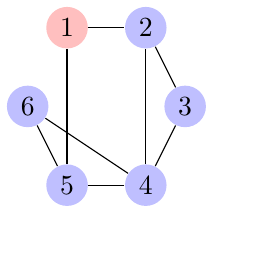
\begin{tikzpicture}[x=0.5cm,y=0.5cm]
    \useasboundingbox (2,-2) rectangle (7.5,3);
    \node[vertexr] (n1) at (3,3)  {1};
    \node[vertexb] (n2) at (5,3)  {2};
    \node[vertexb] (n3) at (6, 1) {3};
    \node[vertexb] (n4) at (5, -1) {4};
    \node[vertexb] (n5) at (3, -1) {5};
    \node[vertexb] (n6) at (2, 1) {6};
    
  
    \foreach \from/\to in {n1/n2,n1/n5,n2/n3,n2/n4,n3/n4,n4/n5,n4/n6,n5/n6}
    \draw (\from) -- (\to);
\end{tikzpicture} \vspace{0.2cm}
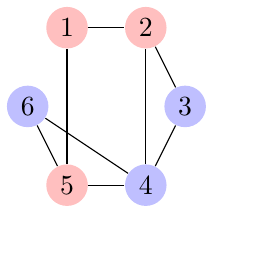
\begin{tikzpicture}[x=0.5cm,y=0.5cm]
    \useasboundingbox (2,-2) rectangle (7.5,3);
    \node[vertexr] (n1) at (3,3)  {1};
    \node[vertexr] (n2) at (5,3)  {2};
    \node[vertexb] (n3) at (6, 1) {3};
    \node[vertexb] (n4) at (5, -1) {4};
    \node[vertexr] (n5) at (3, -1) {5};
    \node[vertexb] (n6) at (2, 1) {6};
    
    \foreach \from/\to in {n1/n2,n1/n5,n2/n3,n2/n4,n3/n4,n4/n5,n4/n6,n5/n6}
    \draw (\from) -- (\to);
\end{tikzpicture} \vspace{0.2cm}
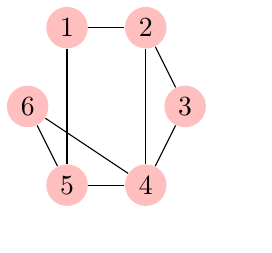
\begin{tikzpicture}[x=0.5cm,y=0.5cm]
    \useasboundingbox (2,-2) rectangle (7.5,3);
    \node[vertexr] (n1) at (3,3)  {1};
    \node[vertexr] (n2) at (5,3)  {2};
    \node[vertexr] (n3) at (6, 1) {3};
    \node[vertexr] (n4) at (5, -1) {4};
    \node[vertexr] (n5) at (3, -1) {5};
    \node[vertexr] (n6) at (2, 1) {6};
    
    \foreach \from/\to in {n1/n2,n1/n5,n2/n3,n2/n4,n3/n4,n4/n5,n4/n6,n5/n6}
    \draw (\from) -- (\to);
\end{tikzpicture} \vspace{0.2cm}

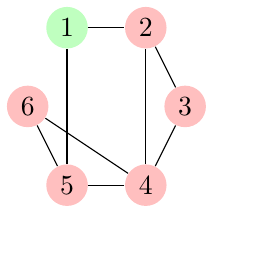
\begin{tikzpicture}[x=0.5cm,y=0.5cm]
    \useasboundingbox (2,-2) rectangle (7.5,3);
    \node[vertexg] (n1) at (3,3)  {1};
    \node[vertexr] (n2) at (5,3)  {2};
    \node[vertexr] (n3) at (6, 1) {3};
    \node[vertexr] (n4) at (5, -1) {4};
    \node[vertexr] (n5) at (3, -1) {5};
    \node[vertexr] (n6) at (2, 1) {6};
    
    \foreach \from/\to in {n1/n2,n1/n5,n2/n3,n2/n4,n3/n4,n4/n5,n4/n6,n5/n6}
    \draw (\from) -- (\to);
\end{tikzpicture} 
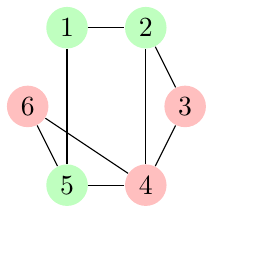
\begin{tikzpicture}[x=0.5cm,y=0.5cm]
    \useasboundingbox (2,-2) rectangle (7.5,3);
    \node[vertexg] (n1) at (3,3)  {1};
    \node[vertexg] (n2) at (5,3)  {2};
    \node[vertexr] (n3) at (6, 1) {3};
    \node[vertexr] (n4) at (5, -1) {4};
    \node[vertexg] (n5) at (3, -1) {5};
    \node[vertexr] (n6) at (2, 1) {6};
    
    \foreach \from/\to in {n1/n2,n1/n5,n2/n3,n2/n4,n3/n4,n4/n5,n4/n6,n5/n6}
    \draw (\from) -- (\to);
\end{tikzpicture} 
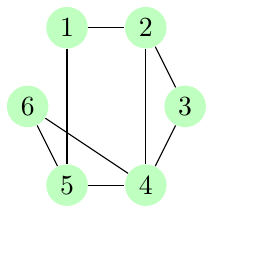
\begin{tikzpicture}[x=0.5cm,y=0.5cm]
    \useasboundingbox (2,-2) rectangle (7.5,3);
    \node[vertexg] (n1) at (3,3)  {1};
    \node[vertexg] (n2) at (5,3)  {2};
    \node[vertexg] (n3) at (6, 1) {3};
    \node[vertexg] (n4) at (5, -1) {4};
    \node[vertexg] (n5) at (3, -1) {5};
    \node[vertexg] (n6) at (2, 1) {6};
    
    \foreach \from/\to in {n1/n2,n1/n5,n2/n3,n2/n4,n3/n4,n4/n5,n4/n6,n5/n6}
    \draw (\from) -- (\to);
\end{tikzpicture} 

\end{center}

\caption{Seqüència d'infeccions amb \begin{math}dI>dR\end{math} (Esquerra a dreta, dalt a baix)}\label{fig4}

\end{figure}

\begin{figure}[h!]
\begin{center}
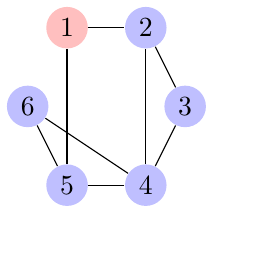
\begin{tikzpicture}[x=0.5cm,y=0.5cm]
    \useasboundingbox (2,-2) rectangle (7.5,3);
    \node[vertexr] (n1) at (3,3)  {1};
    \node[vertexb] (n2) at (5,3)  {2};
    \node[vertexb] (n3) at (6, 1) {3};
    \node[vertexb] (n4) at (5, -1) {4};
    \node[vertexb] (n5) at (3, -1) {5};
    \node[vertexb] (n6) at (2, 1) {6};
    
  
    \foreach \from/\to in {n1/n2,n1/n5,n2/n3,n2/n4,n3/n4,n4/n5,n4/n6,n5/n6}
    \draw (\from) -- (\to);
\end{tikzpicture} \vspace{0.2cm}
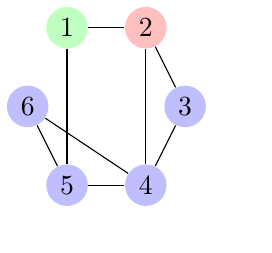
\begin{tikzpicture}[x=0.5cm,y=0.5cm]
    \useasboundingbox (2,-2) rectangle (7.5,3);
    \node[vertexg] (n1) at (3,3)  {1};
    \node[vertexr] (n2) at (5,3)  {2};
    \node[vertexb] (n3) at (6, 1) {3};
    \node[vertexb] (n4) at (5, -1) {4};
    \node[vertexb] (n5) at (3, -1) {5};
    \node[vertexb] (n6) at (2, 1) {6};
    
    \foreach \from/\to in {n1/n2,n1/n5,n2/n3,n2/n4,n3/n4,n4/n5,n4/n6,n5/n6}
    \draw (\from) -- (\to);
\end{tikzpicture} \vspace{0.2cm}
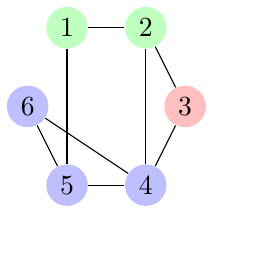
\begin{tikzpicture}[x=0.5cm,y=0.5cm]
    \useasboundingbox (2,-2) rectangle (7.5,3);
    \node[vertexg] (n1) at (3,3)  {1};
    \node[vertexg] (n2) at (5,3)  {2};
    \node[vertexr] (n3) at (6, 1) {3};
    \node[vertexb] (n4) at (5, -1) {4};
    \node[vertexb] (n5) at (3, -1) {5};
    \node[vertexb] (n6) at (2, 1) {6};
    
    \foreach \from/\to in {n1/n2,n1/n5,n2/n3,n2/n4,n3/n4,n4/n5,n4/n6,n5/n6}
    \draw (\from) -- (\to);
\end{tikzpicture} \vspace{0.2cm}
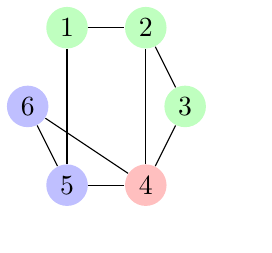
\begin{tikzpicture}[x=0.5cm,y=0.5cm]
    \useasboundingbox (2,-2) rectangle (7.5,3);
    \node[vertexg] (n1) at (3,3)  {1};
    \node[vertexg] (n2) at (5,3)  {2};
    \node[vertexg] (n3) at (6, 1) {3};
    \node[vertexr] (n4) at (5, -1) {4};
    \node[vertexb] (n5) at (3, -1) {5};
    \node[vertexb] (n6) at (2, 1) {6};
    
    \foreach \from/\to in {n1/n2,n1/n5,n2/n3,n2/n4,n3/n4,n4/n5,n4/n6,n5/n6}
    \draw (\from) -- (\to);
\end{tikzpicture} \vspace{0.2cm}

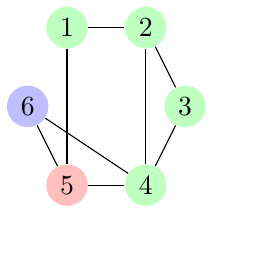
\begin{tikzpicture}[x=0.5cm,y=0.5cm]
    \useasboundingbox (2,-2) rectangle (7.5,3);
    \node[vertexg] (n1) at (3,3)  {1};
    \node[vertexg] (n2) at (5,3)  {2};
    \node[vertexg] (n3) at (6, 1) {3};
    \node[vertexg] (n4) at (5, -1) {4};
    \node[vertexr] (n5) at (3, -1) {5};
    \node[vertexb] (n6) at (2, 1) {6};
    
    \foreach \from/\to in {n1/n2,n1/n5,n2/n3,n2/n4,n3/n4,n4/n5,n4/n6,n5/n6}
    \draw (\from) -- (\to);
\end{tikzpicture} 
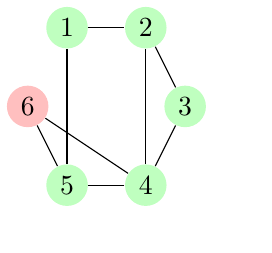
\begin{tikzpicture}[x=0.5cm,y=0.5cm]
    \useasboundingbox (2,-2) rectangle (7.5,3);
    \node[vertexg] (n1) at (3,3)  {1};
    \node[vertexg] (n2) at (5,3)  {2};
    \node[vertexg] (n3) at (6, 1) {3};
    \node[vertexg] (n4) at (5, -1) {4};
    \node[vertexg] (n5) at (3, -1) {5};
    \node[vertexr] (n6) at (2, 1) {6};
    
    \foreach \from/\to in {n1/n2,n1/n5,n2/n3,n2/n4,n3/n4,n4/n5,n4/n6,n5/n6}
    \draw (\from) -- (\to);
\end{tikzpicture} 
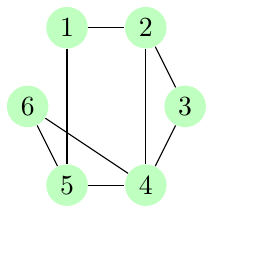
\begin{tikzpicture}[x=0.5cm,y=0.5cm]
    \useasboundingbox (2,-2) rectangle (7.5,3);
    \node[vertexg] (n1) at (3,3)  {1};
    \node[vertexg] (n2) at (5,3)  {2};
    \node[vertexg] (n3) at (6, 1) {3};
    \node[vertexg] (n4) at (5, -1) {4};
    \node[vertexg] (n5) at (3, -1) {5};
    \node[vertexg] (n6) at (2, 1) {6};
    
    \foreach \from/\to in {n1/n2,n1/n5,n2/n3,n2/n4,n3/n4,n4/n5,n4/n6,n5/n6}
    \draw (\from) -- (\to);
\end{tikzpicture} 

\end{center}

\caption{Seqüència d'infeccions amb \begin{math}dI=dR\end{math} (Esquerra a dreta, dalt a baix)}\label{fig5}

\end{figure}

\begin{figure}[h!]
\begin{center}
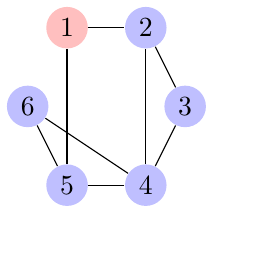
\begin{tikzpicture}[x=0.5cm,y=0.5cm]
    \useasboundingbox (2,-2) rectangle (7.5,3);
    \node[vertexr] (n1) at (3,3)  {1};
    \node[vertexb] (n2) at (5,3)  {2};
    \node[vertexb] (n3) at (6, 1) {3};
    \node[vertexb] (n4) at (5, -1) {4};
    \node[vertexb] (n5) at (3, -1) {5};
    \node[vertexb] (n6) at (2, 1) {6};
    
  
    \foreach \from/\to in {n1/n2,n1/n5,n2/n3,n2/n4,n3/n4,n4/n5,n4/n6,n5/n6}
    \draw (\from) -- (\to);
\end{tikzpicture} 
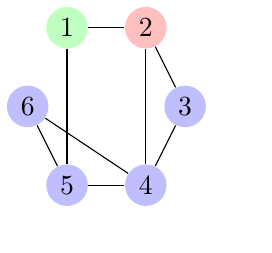
\begin{tikzpicture}[x=0.5cm,y=0.5cm]
    \useasboundingbox (2,-2) rectangle (7.5,3);
    \node[vertexg] (n1) at (3,3)  {1};
    \node[vertexr] (n2) at (5,3)  {2};
    \node[vertexb] (n3) at (6, 1) {3};
    \node[vertexb] (n4) at (5, -1) {4};
    \node[vertexb] (n5) at (3, -1) {5};
    \node[vertexb] (n6) at (2, 1) {6};
    
    \foreach \from/\to in {n1/n2,n1/n5,n2/n3,n2/n4,n3/n4,n4/n5,n4/n6,n5/n6}
    \draw (\from) -- (\to);
\end{tikzpicture} 
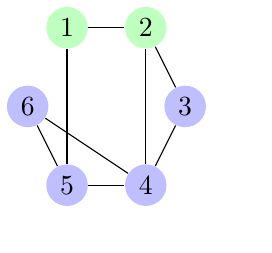
\begin{tikzpicture}[x=0.5cm,y=0.5cm]
    \useasboundingbox (2,-2) rectangle (7.5,3);
    \node[vertexg] (n1) at (3,3)  {1};
    \node[vertexg] (n2) at (5,3)  {2};
    \node[vertexb] (n3) at (6, 1) {3};
    \node[vertexb] (n4) at (5, -1) {4};
    \node[vertexb] (n5) at (3, -1) {5};
    \node[vertexb] (n6) at (2, 1) {6};
    
    \foreach \from/\to in {n1/n2,n1/n5,n2/n3,n2/n4,n3/n4,n4/n5,n4/n6,n5/n6}
    \draw (\from) -- (\to);
\end{tikzpicture} 


\end{center}

\caption{Seqüència d'infeccions amb \begin{math}dI<dR\end{math} (Esquerra a dreta)}\label{fig6}

\end{figure}

\pagebreak

\subsection{SIRV}
\noindent En el nostre cas, utilitzarem un model una mica més complex que el SIR. Afegirem un paràmetre de població vacunada, on el grup estarà immunitzat de l'agent infecciós sense haver de passar la malaltia. Com en el model base haurem de fer algunes suposicions: la vacuna serà 100\% efectiva i no perdrà mai efectivitat i la vacunació de la població començarà a t=0 i seguirà un ritme constant. Aquest nou model s'anomena SIRV.
\smallbreak
\noindent Al igual que el model base, aquest també està format per EDOs i és determinista. Es fan les mateixes assumpcions que al model SIR. \begin{math}\beta\end{math} i \begin{math}\gamma\end{math} tenen les mateixes definicions. A més a més, s’introduex el valor v que simbolitza el percentatge de població susceptible que es vacuna per unitat de temps.
\smallbreak

\begin{math}\frac{dS}{dt}=-\beta SI\end{math}

\begin{math}\frac{dI}{dt}=\beta SI - \gamma I\end{math}

\begin{math}\frac{dR}{dt}=\gamma I\end{math}

\begin{math}\frac{dV}{dt}=vS\end{math}

\pagebreak

\noindent Com es pot veure a les Fig 8 i 9, com més gran sigui v, menys temps es tardarà a vacunar a una població. I, per tant, serà més difícil que un brot esdevingui una pandèmia, ja que no hi haurà tants individus susceptibles que es puguin contagiar.

\begin{figure}[h]
\begin{center}
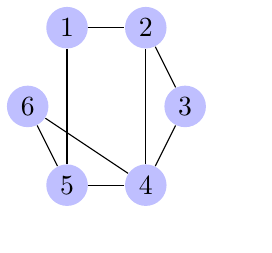
\begin{tikzpicture}[x=0.5cm,y=0.5cm]
    \useasboundingbox (2,-2) rectangle (7.5,3);
    \node[vertexb] (n1) at (3,3)  {1};
    \node[vertexb] (n2) at (5,3)  {2};
    \node[vertexb] (n3) at (6, 1) {3};
    \node[vertexb] (n4) at (5, -1) {4};
    \node[vertexb] (n5) at (3, -1) {5};
    \node[vertexb] (n6) at (2, 1) {6};
    
  
    \foreach \from/\to in {n1/n2,n1/n5,n2/n3,n2/n4,n3/n4,n4/n5,n4/n6,n5/n6}
    \draw (\from) -- (\to);
\end{tikzpicture}
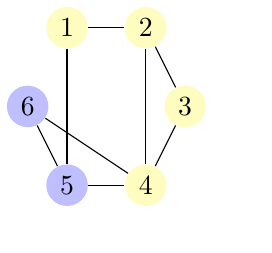
\begin{tikzpicture}[x=0.5cm,y=0.5cm]
    \useasboundingbox (2,-2) rectangle (7.5,3);
    \node[vertexy] (n1) at (3,3)  {1};
    \node[vertexy] (n2) at (5,3)  {2};
    \node[vertexy] (n3) at (6, 1) {3};
    \node[vertexy] (n4) at (5, -1) {4};
    \node[vertexb] (n5) at (3, -1) {5};
    \node[vertexb] (n6) at (2, 1) {6};
    
    \foreach \from/\to in {n1/n2,n1/n5,n2/n3,n2/n4,n3/n4,n4/n5,n4/n6,n5/n6}
    \draw (\from) -- (\to);
\end{tikzpicture} 
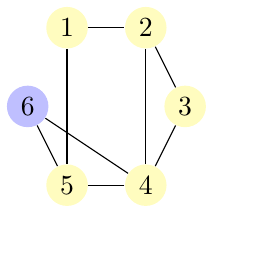
\begin{tikzpicture}[x=0.5cm,y=0.5cm]
    \useasboundingbox (2,-2) rectangle (7.5,3);
    \node[vertexy] (n1) at (3,3)  {1};
    \node[vertexy] (n2) at (5,3)  {2};
    \node[vertexy] (n3) at (6, 1) {3};
    \node[vertexy] (n4) at (5, -1) {4};
    \node[vertexy] (n5) at (3, -1) {5};
    \node[vertexb] (n6) at (2, 1) {6};
    
    \foreach \from/\to in {n1/n2,n1/n5,n2/n3,n2/n4,n3/n4,n4/n5,n4/n6,n5/n6}
    \draw (\from) -- (\to);
\end{tikzpicture} 
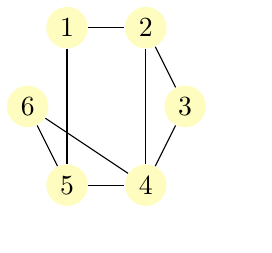
\begin{tikzpicture}[x=0.5cm,y=0.5cm]
    \useasboundingbox (2,-2) rectangle (7.5,3);
    \node[vertexy] (n1) at (3,3)  {1};
    \node[vertexy] (n2) at (5,3)  {2};
    \node[vertexy] (n3) at (6, 1) {3};
    \node[vertexy] (n4) at (5, -1) {4};
    \node[vertexy] (n5) at (3, -1) {5};
    \node[vertexy] (n6) at (2, 1) {6};
    
    \foreach \from/\to in {n1/n2,n1/n5,n2/n3,n2/n4,n3/n4,n4/n5,n4/n6,n5/n6}
    \draw (\from) -- (\to);
\end{tikzpicture} 

\end{center}

\caption{Seqüència de vacunació amb v=\begin{math}\frac{2}{3}\end{math} (Esquerra a dreta)}

\end{figure}

\begin{figure}[h]
\begin{center}
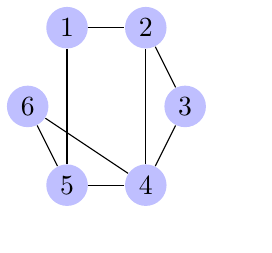
\begin{tikzpicture}[x=0.5cm,y=0.5cm]
    \useasboundingbox (2,-2) rectangle (7.5,3);
    \node[vertexb] (n1) at (3,3)  {1};
    \node[vertexb] (n2) at (5,3)  {2};
    \node[vertexb] (n3) at (6, 1) {3};
    \node[vertexb] (n4) at (5, -1) {4};
    \node[vertexb] (n5) at (3, -1) {5};
    \node[vertexb] (n6) at (2, 1) {6};
    
  
    \foreach \from/\to in {n1/n2,n1/n5,n2/n3,n2/n4,n3/n4,n4/n5,n4/n6,n5/n6}
    \draw (\from) -- (\to);
\end{tikzpicture}
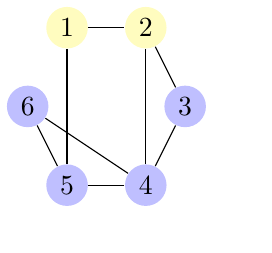
\begin{tikzpicture}[x=0.5cm,y=0.5cm]
    \useasboundingbox (2,-2) rectangle (7.5,3);
    \node[vertexy] (n1) at (3,3)  {1};
    \node[vertexy] (n2) at (5,3)  {2};
    \node[vertexb] (n3) at (6, 1) {3};
    \node[vertexb] (n4) at (5, -1) {4};
    \node[vertexb] (n5) at (3, -1) {5};
    \node[vertexb] (n6) at (2, 1) {6};
    
    \foreach \from/\to in {n1/n2,n1/n5,n2/n3,n2/n4,n3/n4,n4/n5,n4/n6,n5/n6}
    \draw (\from) -- (\to);
\end{tikzpicture} 
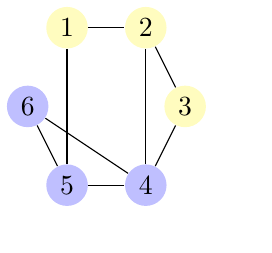
\begin{tikzpicture}[x=0.5cm,y=0.5cm]
    \useasboundingbox (2,-2) rectangle (7.5,3);
    \node[vertexy] (n1) at (3,3)  {1};
    \node[vertexy] (n2) at (5,3)  {2};
    \node[vertexy] (n3) at (6, 1) {3};
    \node[vertexb] (n4) at (5, -1) {4};
    \node[vertexb] (n5) at (3, -1) {5};
    \node[vertexb] (n6) at (2, 1) {6};
    
    \foreach \from/\to in {n1/n2,n1/n5,n2/n3,n2/n4,n3/n4,n4/n5,n4/n6,n5/n6}
    \draw (\from) -- (\to);
\end{tikzpicture} 
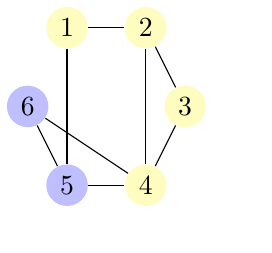
\begin{tikzpicture}[x=0.5cm,y=0.5cm]
    \useasboundingbox (2,-2) rectangle (7.5,3);
    \node[vertexy] (n1) at (3,3)  {1};
    \node[vertexy] (n2) at (5,3)  {2};
    \node[vertexy] (n3) at (6, 1) {3};
    \node[vertexy] (n4) at (5, -1) {4};
    \node[vertexb] (n5) at (3, -1) {5};
    \node[vertexb] (n6) at (2, 1) {6};
    
    \foreach \from/\to in {n1/n2,n1/n5,n2/n3,n2/n4,n3/n4,n4/n5,n4/n6,n5/n6}
    \draw (\from) -- (\to);
\end{tikzpicture} 

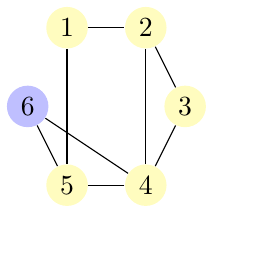
\begin{tikzpicture}[x=0.5cm,y=0.5cm]
    \useasboundingbox (2,-2) rectangle (7.5,3);
    \node[vertexy] (n1) at (3,3)  {1};
    \node[vertexy] (n2) at (5,3)  {2};
    \node[vertexy] (n3) at (6, 1) {3};
    \node[vertexy] (n4) at (5, -1) {4};
    \node[vertexy] (n5) at (3, -1) {5};
    \node[vertexb] (n6) at (2, 1) {6};
    
    \foreach \from/\to in {n1/n2,n1/n5,n2/n3,n2/n4,n3/n4,n4/n5,n4/n6,n5/n6}
    \draw (\from) -- (\to);
\end{tikzpicture} 
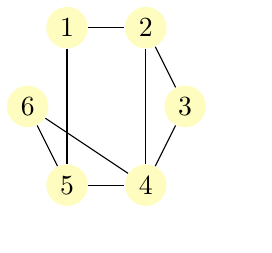
\begin{tikzpicture}[x=0.5cm,y=0.5cm]
    \useasboundingbox (2,-2) rectangle (7.5,3);
    \node[vertexy] (n1) at (3,3)  {1};
    \node[vertexy] (n2) at (5,3)  {2};
    \node[vertexy] (n3) at (6, 1) {3};
    \node[vertexy] (n4) at (5, -1) {4};
    \node[vertexy] (n5) at (3, -1) {5};
    \node[vertexy] (n6) at (2, 1) {6};
    
    \foreach \from/\to in {n1/n2,n1/n5,n2/n3,n2/n4,n3/n4,n4/n5,n4/n6,n5/n6}
    \draw (\from) -- (\to);
\end{tikzpicture} 

\end{center}

\caption{Seqüència de vacunació amb v=\begin{math}\frac{1}{3}\end{math} (Esquerra a dreta, dalt a baix)}

\end{figure}
\pagebreak
\section{Aplicacions}
\medbreak
Aquest model va ser creat per tenir alguna manera de predir el número i la distribució d’una enfermetat infecciosa a mesura que es transmet a través de la població al llarg del temps.
Tot i aquest propòsit inicial, actualment té diferents aplicacions que s’exposarán més endavant.
\medbreak
Per entendre les seves aplicacions cal conèixer algunes de les seves limitacions :
\begin{itemize}
    \item És un model bàsic on s’assumeix una població tancada, el que significa que no hi ha naixements,morts naturals o viatges dins la població
    \item Es considera a la població com a una barreja homogènia, per tant que qualsevol persona del món té les mateixes possibilitats d’actuar amb qualsevol altre persona del món
    \item El model assumeix que no hi ha períodes latents o inactius, ni la possibilitat de mutació viral.
\end{itemize}
\medbreak
La senzillesa d’aquest model permet una modulació prèvia de  l’evolució de qualsevol pandèmia sense necessitat de conèixer masses paràmetres i amb càlculs matemàtics poc avançats. És per això que ’aplicació d’aquest model está pensada per a períodes no gaire prolongats en el temps, ja que no contempla tots els paràmetres de morts i naixaments de la població. Per la qual cosa, si es vol contemplar un període considerable de temps és recomenable afegir altres parámetres sobre la variació natural de la població.
\medbreak

Un cop conegut el funcionament basic i les seves limitacions podem destacar-ne algunes aplicacions.
\medbreak

\textbf{Principal Aplicació: Epidemiologia}
\medbreak
Com bé s’ha detallat a la pàgina anterior, la raó per la qual fou creat el SIR model va ser per obtenir un model matemàtic eficient per a la predicció de l’evolució del comportament i impacte d’un virus a la societat.
\medbreak
Utilitzar models matemàtics per estudiar el comportament d’enfermetats infeccioses és de vital importància per a la població, ja que si es coneix la tendència que segueix la propagació del virus amb antelació la societat pot idear tot tipus de mesures per a intentar contrarestar el virus de la manera més òptima possible.
\medbreak
Per a veure un exemple recent de l'ús del model en el desenvolupament d'una pandèmia s'ha adjuntat el següent gràfic on es pot veure la idea bàsica de l'aplicació del model SIR per a la modelació del Covid-19 a Santa Marta, Colòmbia. 
Observem la projecció del nombre de susceptibles, infectats i recuperats des de l'inici de la pandèmia, del 20 de març del 2020 fins a l'1 de gener del 2022.

\begin{figure}[h!]
    \centering
    \includegraphics[width=0.5\linewidth]{image1.png}
    \caption{ Modelació del Covid-19 a Santa Marta, Colòmbia. Infectats, susceptibles i recuperats des de l'inici de la pandèmia , del 20 de març del 2020 fins a l'1 de gener del 2022} 

\cite{grafic1}
\end{figure}

\pagebreak

A part del covid, el model SIR es porta utilitzant des de el 1920 en altres epidèmies i també per a la comparació d’aquestes. Per tant, aquest model diferencial veiem que és molt útil tant per la predicció del desenvolupament de les pandèmies com per la comparació de danys i implicacions a la societat. 
\medbreak
\textbf{Altres aplicacions}
\medbreak
Tot i que el model SIR és àmpliament utilitzat en epidemiologia per modelar la propagació de malalties infeccioses, també té usos en altres camps. 
A continuació vaurem quines són algunes de les aplicacions dels models matemàtics diferencials com pot ser el SIR:
\medbreak
\textbf{Dinàmica de poblacions}: Per estudiar la dinàmica de poblacions en ecologia, com la propagació d'espècies invasores en un ecosistema o la difusió de comportaments socials entre individus.
\medbreak
\textbf{Difusió d'informació i rumors:} En l'àmbit de les xarxes socials i la comunicació, el model SIR es pot aplicar per entendre com es propaga la informació, els rumors o les tendències a través d'una població.
\medbreak
\textbf{Productes i màrqueting}: En l'àmbit empresarial, es poden aplicar per entendre com es propaguen els productes, les modes o les estratègies de màrqueting entre els consumidors.
\medbreak
\textbf{Difusió política }: Per modelar la difusió d'opinions, creences o tendències polítiques i socials dins d'una comunitat.


\clearpage

\section{Anàlisis}
\subsection{Anàlisis control}
En aquest anàlisis veurem una gràfica una infecció (sense tindre en compte la vacunació) amb les següents dades inicials:\cite{mathlab}

\begin{itemize}
    \item \begin{math}\beta = 5*10^-9\end{math}; tasa de infecció a la epidèmia
    \item \begin{math}gamma = 0.12\end{math}; tasa de recuperació a la epidèmia
    \item \begin{math}delta = 0.0\end{math}; tasa de pèrdua de la inmunitat a la epidèmia
    \item \begin{math}N = 6*10^7\end{math}; nombre de la població total (S + I + R)
    \item $S$; Nombre de persones susceptibles a la epidèmia
    \item $I$; Nombre de persones infectades per la epidèmia
    \item $R$; Nombre de persones que s'han recuperat de la epidèmia
    \item $I0 = 10$; nombre inicial de infectats
    \item $T = 300$; periode total de temps (300 dies)
    \item $dt = 1/4$; interval de temps expressat en un quart de dia
\end{itemize}
\medbreak
\textit{Hem escollit que la delta, el percentatge que indica la probabilitat de perdre la immunitat un cop una persona es recupera de la infecció, sigui 0 per simplificar els càlculs i resultats.}

\begin{figure}[h!]
    \centering
    \includegraphics[scale=0.2]{grafica 300 dies.jpg}
    \caption{Control (T=300 dies)}
    \label{fig:enter-label}
    \cite{mathlab}
\end{figure}


\subsubsection{Conclusions}
Com podem apreciar en la Fig. 11, aquest model concret podem veure que el curs normal de una epidèmia es que a mesura que la població infectada (I) va augmentant, la població susceptible (S) vagi disminuint significativament. També, com hi han infectats, les persones es comencen a recuperar i així la població que s’ha recuperat de la malaltia (R) va augmentant també. Si ens fixem més, podem distingir que quan hi ha el pic de persones infectades, és quan hi també el màxim creixement de la població (R) i un màxim decreixement en la població (S). Aquest fet és totalment lògic i esperable, doncs te sentit pensar que quantes més persones infectades, més persones tindran la probabilitat de recuperar-se. També, de les equacions\cite{siruab} podem deduir que el nombre màxim d'infectats es donarà quan el nombre de susceptibles S(t) = 1/Ro. Per tal d'assolir la immunitat de ramat el nombre d'individus recuperats haurà de ser major a 26000000 milions de persones (52 \% de la població).

\subsection{Anàlisis amb confinament}
Per simular un confinament bastarà si modifiquem el paràmetre (tau) que es la variable que determina el contacte entre les persones en la epidèmia.\cite{siruab} Així doncs, com la beta es descriu per la següent equació:
\medbreak
\begin{math}
    \beta = \frac{b}{N}\end{math} on b=\begin{math}\kappa*\tau
\end{math}\cite{siruab}
\medbreak
On \begin{math}\beta\end{math} és la tasa de infecció, \begin{math}\tau\end{math} és la transmissibilitat (\textit{transmissibility})\cite{siruab} entre persones durant la epidèmia i \begin{math}\kappa\end{math} és el nombre de contactes entre persones durant la epidèmia.
\par
Podem reduir la \begin{math}\kappa\end{math} en un 90\% aplicant un factor de 1/10 en  l’equació quedant de la següent manera:
\medbreak
\begin{math}\beta_{confinament} = 1/10 * \beta_{pre-confinament}
\end{math}\cite{siruab}
\medbreak
En aquest anàlisis utilitzarem les dades del control però iniciarem un confinament als 80 dies (quan T = 120 ). Per crear això farem dos simulacions una amb les dades de la simulació 1.1 però reduint el temps total T a 80 dies. I una segona simulació amb les dades inicials iguals a les dades finals de la primera simulació i aplicant el canvi en el paràmetre beta per simular el confinament. (Per simplificar càlculs només utilitzarem el nombre de infectats final de la primera simulació com el nombre de infectats inicials de la segona, I0).

\begin{figure}[h!]
    \centering
    \includegraphics[scale=0.2]{grafica (80 dies).jpg}
    \caption{Simulació pre-confinament (T=80) ; \begin{math}\beta_{pre-confinament}\end{math}}
    \label{fig:enter-label}
    \cite{mathlab}
\end{figure}

\begin{figure}[h!]
    \centering
    \includegraphics[scale=0.2]{grafica I (80 dies).jpg}
    \caption{Total de persones infectades en els 80 dies de pre-confinament}
    \label{fig:enter-label}
    \cite{mathlab}
\end{figure}

\begin{figure}[h!]
    \centering
    \includegraphics[scale=0.2]{grafica 220 dies.jpg}
    \caption{Simulació aplicant el confinament (T=220 ; \begin{math}\beta_{confinament} = 1/10 * \beta_{pre-confinament}\end{math})}
    \label{fig:enter-label}
    \cite{mathlab}
\end{figure}

\pagebreak

\subsubsection{Conclusions}
Com podem veure en les figures 12,13 i 14, al aplicar el confinament la corba d’infectats ha disminuït significativament més ràpid. Doncs amb el confinament les persones tenen menys probabilitats de interactuar i per tant de infectar-se (considerant que en aquesta epidèmia el contacte o la exposició amb persones infectades és necessària per infectar-se.
\pagebreak
\section{Vacunació}


\noindent \textit{" Vaccinating an entire population is very expensive, and not everybody can take the vaccine. Some individuals, such as those with compromised immune systems or severe allergies, the vaccine may be worse than the disease"}~\cite{siruab} . L'objectiu a assolir és el que es coneix com la immunitat de ramat. "The notion of herd immunity is simple, yet profound: not every member of a population must be immune to prevent large-scale outbreaks, nor will everyone be infected during the course of an epidemic"~\cite{herdimmunity}. S'haurà aconseguit la immunitat de ramat una vegada hi hagi una determinada part de la població que no pugui ser infectada.\medbreak

\begin{figure}[h!]
    \centering
    \includegraphics[width=0.9\linewidth]{inmunidad.PNG}
    \caption{Representació d'inmunitat de grup~\cite{herdimmunity}}
    \label{fig:enter-label}
\end{figure}

\noindent Com veiem a la figura 15, podem diferenciar tres fases en el transcurs d'una pandèmia. Inicialment (A) tindrem un primer individu infectat que es troba en una població d'individus no immunitzats. L'individu infectat tindrà contacte amb els susceptibles i aquesta cadena de contacte entre infectat i susceptible serà el detonant d'una pandèmia. Després d'un cert temps (B) alguns individus desenvoluparan immunitat. Això comportarà que el nombre de contactes entre infectats i susceptibles es veurà reduït. Finalment, (C) la proporció d'individus recuperats serà suficient per assolir la immunitat de ramat.\medbreak

\noindent La qüestió que ens plantegem a continuació fa referència al problema de determinar quina serà la part dels individus susceptibles que hauran de ser vacunats per arribar a la immunitat de ramat. En aquest model, l'acció de vacunar es tradueix a fer que una persona passi de susceptible a recuperat sense haver de passar per la classe d'infectat. A l'apartat 1 \textit{(MODEL SIR "Pag. 3")} s'ha discutit com el nombre reproductiu efectiu (Re) pot ser un punt d'inflexió en el curs d'una pandèmia. Recordem que quan Re > 1 el nombre d'infectats decreixerà fins a arribar a 0 per \(t\rightarrow \infty\), mentre que si Re > 1 el nombre d'infectats creixerà fins a arribar a un pic, després tendirà a 0 per \(t\rightarrow \infty\). ~\cite{siruab}
\bigbreak
\noindent Establim la condicio \(R_e\) \leq 1:



\midbreak

\begin{math}
    S'(0)\frac{\beta}{\gamma} \leq 1
\end{math}

\midbreak

\begin{math}
    (S(0) - R)\frac{\beta}{\gamma} \leq 1
\end{math}

\midbreak

\begin{math}
    R \geq (S(0) - \frac{\gamma}{\beta})
\end{math}

\noindent Hem de tenir en compte que ara S'(0) no es N - I(0) sinó que, S'(0) = S(0) - R. Definim R com el nombre de persones recuperades, entre aquestes s'inclouen les persones vacunades i les que després de ser infectades s'han recuperat. Notem que per un \(R_e\) més gran necessitarem un major nombre de recuperats.\bigbreak



\begin{figure}[h!]
    \centering
    \includegraphics[scale=0.3]{figura1.png}
    \caption{Control (T=300dies , Tassa de vacunació v = 0)}
    \label{fig:enter-label}
    \cite{odesolver}
\end{figure}

\noindent En la figura 16 s'observa l'evolució d'una pandèmia on la tassa de vacunació v és igual a 0. És a dir el cas en el qual no vacunem a la població. Si calculem el Re, obtenim un valor de 2.083. Podem veure com hi haurà un pic d'infeccions al voltant dels cent vint dies amb un nombre màxim d'infectats de 14 millons de persones.



\begin{figure}[h!]
    \centering
    \includegraphics[scale=0.3]{figura2.png}
    \caption{Tassa de vacunació v = 0.005}
    \label{fig:enter-label}
    \cite{odesolver}
\end{figure}


\noindent En la figura 17 introduïm una tassa de vacunació v = 0.005. Podem apreciar una reducció significativa en el pic d'infectats amb un nombre màxim d'infectats al voltant d'1.8 milions. És evident que la incorporació de les vacunes avantatge un desenvolupament favorable de la pandèmia. Del gràfic s'observa com més individus es recuperen sense ser infectats prèviament. Això contribueix al control de la població infectada. S'ha calculat anteriorment que el nombre de recuperats haurà de ser major als 36000000 per arribar a la immunitat de grup. Gràcies a la vacunació, s'aconsegueix aquest nombre de formes més fàcil, ja que ara haurem de considerar com a recuperats aquells que ho són per vacunació i els que ho són per infecció.

\bigbreak


\begin{figure}[h!]
    \centering
    \includegraphics[scale=0.3]{figura3.png}
    \caption{Tassa de vacunació v = 0.007}
    \label{fig:enter-label}
    \cite{odesolver}
\end{figure}

\bigbreak

\noindent Si augmentem la tassa de vacunació, el nombre d'infectats gairebé no varia respecte a la població inicial d'infectats (I0). Aquesta manté un valor quasi constant fins que tendeix a 0 a l'infinit. Directament, podem concloure que una tassa de vacunació adient fa que puguem prendre control sobre la pandèmia.


\bigbreak

\noindent A continuació estudiem únicament l'evolució dels individus recuperats per infecció i els recuperats per vacunació. Inicialment, els dos grups creixen, però arriba un cert instant en què els recuperats de forma natural s'estabilitzen mentre que el grup dels vacunats continua augmentant. Quina explicació podem donar a aquest fet?

\bigbreak

\begin{figure}[b]
    \centering
    \includegraphics[scale=0.3]{figura4.png}
    \caption{Comparació dels individus recuperats per vacunació i els recuperats de forma natural.}
    \label{fig:enter-label}
    \cite{odesolver}
\end{figure}



\noindent El causant d'aquesta diferència en el creixement dels dos grups està directament relacionat amb l'impacte de la vacunació sobre una població. Si analitzem el resultat obtingut, és obvi que a mesura que el nombre d'individus vacunats s'intensifica, el nombre d'individus susceptibles decreixerà. Com més gran sigui la tassa de vacunació, més accentuat serà aquest decreixement. Aquest succés es torna evident quan un mira les equacions que regeixen el model. Un nombre menor d'individus susceptibles, provocarà un menor nombre d'infeccions i, per tant, també menys recuperats de forma natural.


\medbreak

\noindent Deixant enrere el model, ens preguntem que tan realista és aquest resultat. Vacunar a la població ens garanteix vèncer a la pandèmia o hi ha altres variables que no hem tingut en compte.

\medbreak

\noindent Existeixen certes condicions que poden fer que es perdi la immunitat de grup. "Even if protection is lifelong, the level of immunity is gradually but inevitably eroded through population turnover. Immune individuals may die from other causes, while births lead to a steady infl ux of newly susceptible hosts (a net immigration of susceptible individuals has a similar effect). As with waning immunity, the population will likely experience repeated epidemic cycles in the absence of interventions". Per altra banda, en alguns casos com en la Covid-19, ens trobem amb mutacions o variants de la mateixa malaltia que poden fer que individus que eren immunes tornin a ser susceptibles.

\medbreak

\noindent En conclusió, com s’esperava els resultats apunten a un clar benefici de les vacunes a l’hora de combatre una pandèmia. Hem vist que seguint el procés de vacunació s’aconsegueix tenir el control de la població infectada i arribar a la immunitat de forma més ràpida i eficient.

\pagebreak
\printbibliography

\end{document}
